\documentclass[12pt]{article}
\usepackage{amsfonts,amssymb}
\usepackage{amsmath}
\usepackage{hyperref}
\usepackage{graphicx}
\usepackage{listings}
\usepackage[autostyle]{csquotes}
%\documentstyle[12pt,amsfonts]{article}
%\documentstyle{article}

\setlength{\topmargin}{-.5in}
\setlength{\oddsidemargin}{0 in}
\setlength{\evensidemargin}{0 in}
\setlength{\textwidth}{6.5truein}
\setlength{\textheight}{8.5truein}
%
%\input ../adgeomcs/lamacb.tex
%\input mac.tex
%\input mathmac.tex
%
\input xy
\xyoption{all}
\def\fseq#1#2{(#1_{#2})_{#2\geq 1}}
\def\fsseq#1#2#3{(#1_{#3(#2)})_{#2\geq 1}}
\def\qleq{\sqsubseteq}
%cis51109hw1

%
\begin{document}
\begin{center}
\fbox{{\Large\bf Functions}}\\
\vspace{1cm}
\end{center}


\medskip\noindent


\vspace{0.5cm}\noindent

\section*{Definition of a relation}

A relation between set $A$ and set $B$ is a subset of $A \times B$. While for the purposes of pure math there does not need to be any underlying property that governs the relation, for most practical purposes, you will find that there will be some property.

For example: Consider the set $A = \{1,2,3\}$ and $B = \{4,5,6\}$ and let us define the relation $R$ to consist of tuples $\{(a,b)| a \in A, b \in B \text{ and } b = a + 3\}$.
Then the relation $R = \{(1,4) , (2,5), (3,6)\}$.

If $(a,b) \in R$, then this is very often denoted as $aRb$.
That notation is similar to the way we write out relations like greater than, less than etc.

\section*{Properties}

\begin{itemize}
\item A relation $R$ on set $A$ is reflexive if \textbf{for all} elements $a$ in set $A$, aRa. 
\item A relation $R$ from set $A$ to set $B$ is said to be symmetric if $aRb$ means that $bRa$ (implicitly we are assuming $a \in A$, $b \in B$).
\item A relation $R$ on a set $A$ is said to be transitive if whenever $aRb$ and $bRc$ then $aRc$. 
\item A relation $R$ is said to be an equivalence relation if and only if it is reflexive, symmetric and transitive.
\item A relation $R$ is said to be anti-symmetric if $aRb$ and $bRa$ can only happen when $a =b$.

Alternatively we can define anti-symmetric as $x \neq y$ should imply that either $x$ is not related to $y$ or $y$ is not related to $x$.

\end{itemize}

\section*{Examples}
\begin{enumerate}
\item Given the set $A = \{1, 2, 4\}$, define the relation $R$ to be the $\le$ relation. That is $aRb$ whenever $a \le b$.

Is this reflexive?  Yes. For $a \le a$ is always true. In particular, it is true for elements of $A$.

Is this symmetric? No. For instance $1 \le 2$ but it is not the case that $2 \le 1$.

Is this transitive? Yes. If $a \le b$ and $ b \le c$ then it is clearly true that $a \le c$.

Is this anti-symmetric? Yes. If $a \le b$ and $b \le a$ then it must be the case that $a = b$.

\item Given the set $U$ = the set of all the states in the USA. 

Let us define a relation as follows. Two states are related if and only if they are adjacent (they share a land or water border). 

Is this reflexive? That is an interesting question because it really depends on the answer to a question like `does Pennsylvania border Pennsylvania'. And really that argument can go both ways. This is a classic case of English and Math not being totally in sync. It is also a reason why after a while, we have to resort to more mathematical examples!

Is this symmetric? This is clear. YES. 

Is this transitive? No. While we have not covered the concept of a mathematical proof yet, it is important to learn that in order to disprove a statement that says `for every ....', all you need to demonstrate is one counter example. Think of it as the one rotten apple!

Where does this fall apart? Virginia borders North Carolina. North Carolina borders South Carolina. But VA does not border SC. 

Is this anti-symmetric? No. The same example as above works as a counter example. 

\end{enumerate}

\medskip

Is it possible for a relation to be symmetric and anti-symmetric at the same time?

This will lead to the concept of a vacuously true statement. 

Consider the set $\{1\}$ and the relation $\{(1,1)\}$. While seemingly trivial and stupid, this relation turns out to be both symmetric and anti-symmetric.


\section*{Definition of a function}

A function $f$ from a set $X$ to a set $Y$, denoted $f : X \rightarrow Y$ is a relation from $X$, the domain
to $Y$ the co-domain that satisfies two properties

\begin{enumerate}
\item every element of $X$ is related to some element in $Y$
\item no element of $X$ is related to more than one element in $Y$
\end{enumerate}

The zybook refers to the co-domain as target. 

The set of all values of  $f$ taken together - range. 

You are probably used to functions in calculus. The functions we do in this course are exactly the same (yay! math definitions do not just change randomly). The big advantage is we can draw what is generally referred as arrow diagrams since the sets we deal with are discrete.

Note:- A function definition is incomplete unless the domain of the function is specified. It is also generally a good idea specify the co-domain, but if not specified it is just considered to be the range of all possible values that the function takes.

Note: - Every function is a relation but only some relations are functions. In particular it is easy to define the relation $R = \{(x, f(x)) \text{ where }  x \in A \}$. 

Here is an example of a relation which is not a function $R = \{(1,1), (1,3)\}$. Why is this not a function? Because 1 is being related to both 1 and 3. To be a function 1 can be mapped to only a single thing!

\section*{Examples}

Here are a few examples of mappings between 2 sets that either are functions or are not functions depending upon the 

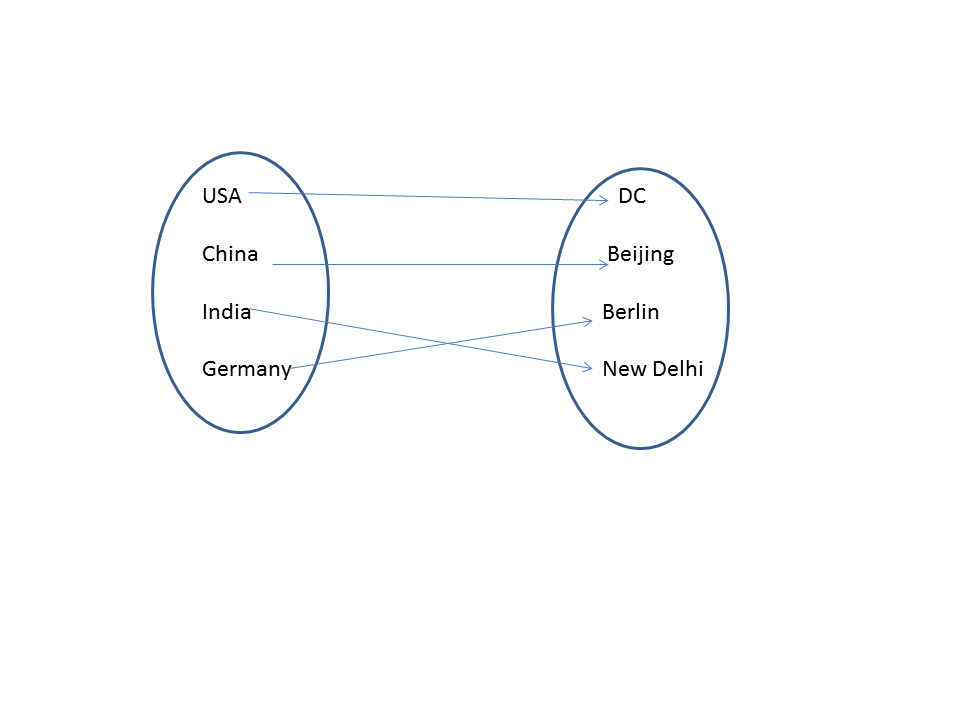
\includegraphics[scale=0.5]{./img/func1.png}

In this first example we are mapping between countries in the left side to the capitals of countries on the right. This is a function because every country has a capital and every country (in this diagram!) has only 1 capital. Trivia: - Name a country that has more than 1 capital.

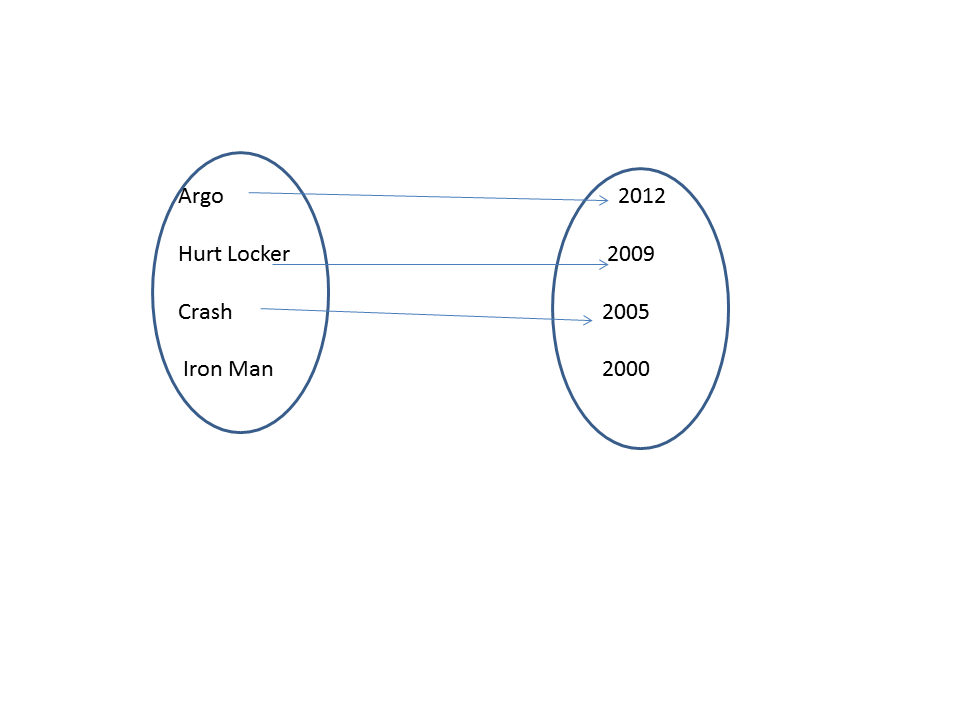
\includegraphics[scale=0.5]{./img/func2.png}

In this second example we are mapping between movies in the left side to years in which they won the best picture award at the oscars. No movie wins the best picture award for more than 1 year, so that condition is satisfied. But Iron Man did not win the best picture award ever, and hence this is not a function.

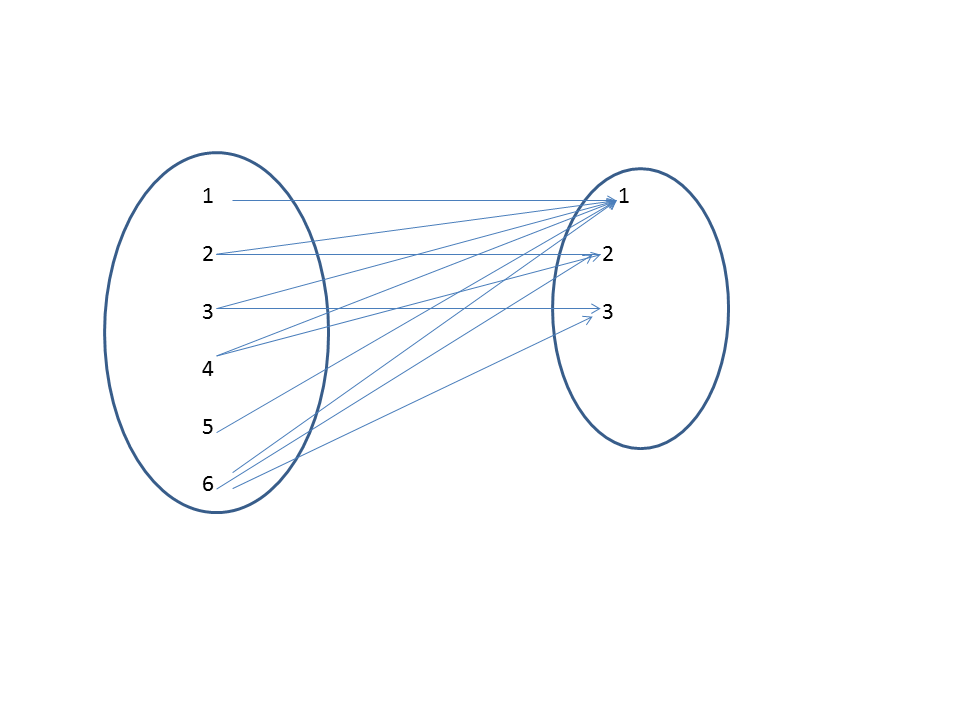
\includegraphics[scale=0.5]{./img/func3.png}

In this third example we have integers from 1 to 6 on the left side and integers from 1 to 3 on the right side. 
The integers in the left set are mapped to integers on the right side if the right integer is a factor of the left integer. Remember that $b$ is a factor of $a$ if $b$ divides $a$. Also recall that $1$ is a factor for every integer.

This example fails to be a function because a number of elements in the left set are being mapped to more than 1 element on the right.

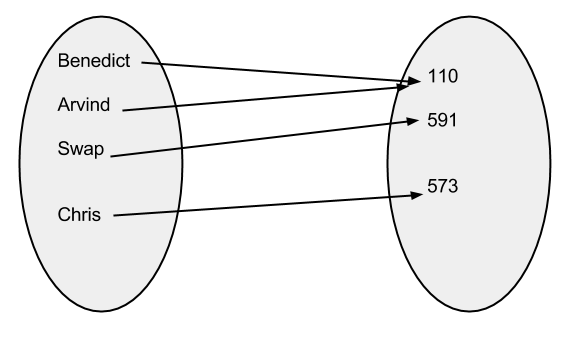
\includegraphics[scale=0.5]{./img/stillAFunc.png}

In this example although both Benedict and Arvind are teaching CIS110, it is still a function! Note that no where in the definition of a function does it say that each element of the first set must be mapped to a different element of the second set.

Two functions $F: X \rightarrow Y$ and $G: X \rightarrow Y$ are said to be equal iff $F(x) = G(x)$ for every $x \in X$.

\subsection*{Ceiling and Floor}
There are a few functions which show up a lot in Computer Science, especially once you start analyzing algorithms. The extremely common one is the log function, which you might have seen before but we will cover in a little bit more detail once we get to analyzing algorithms.
Two others which are used extensively to approximate things are the ceiling and the floor function.

The ceiling function, denoted as $\lceil x \rceil$, is the smallest integer $y$ such that $y \ge x$. 

The floor function, denoted as $\lfloor x \rfloor$ is the greatest integer $y$ such that $y \le x$.

\medskip

Is the floor function defined on $\mathbb{R}$ one-one? 
When a statement like the above one is made, the implicit assumption is that both the domain and the co-domain are $\mathbb{R}$. 

Consider these two $\lfloor \pi \rfloor$ and $\lfloor 3.5 \rfloor$. They are both 3! So here we have two distinct element of $\mathbb{R}$ mapping to the same element. The floor function is not one-one on $\mathbb{R}$.

\medskip

Is the floor function defined on $\mathbb{Z}$ one-one?
This function IS one-one because what is the floor of any integer? It is the integer itself!
So you will not have the previous situation. 

\section*{One-One}
A function is said to be one to one if $x \neq y$ means $f(x) \neq f(y)$. Equivalently, 
$f(x) = f(y)$ means $x = y$. 

Of the two functions above, which is one to one. 

From an arrow-diagram identifying whether a function is one-one is immediate. You just have to make sure that you do not have two arrow heads incident on the same point

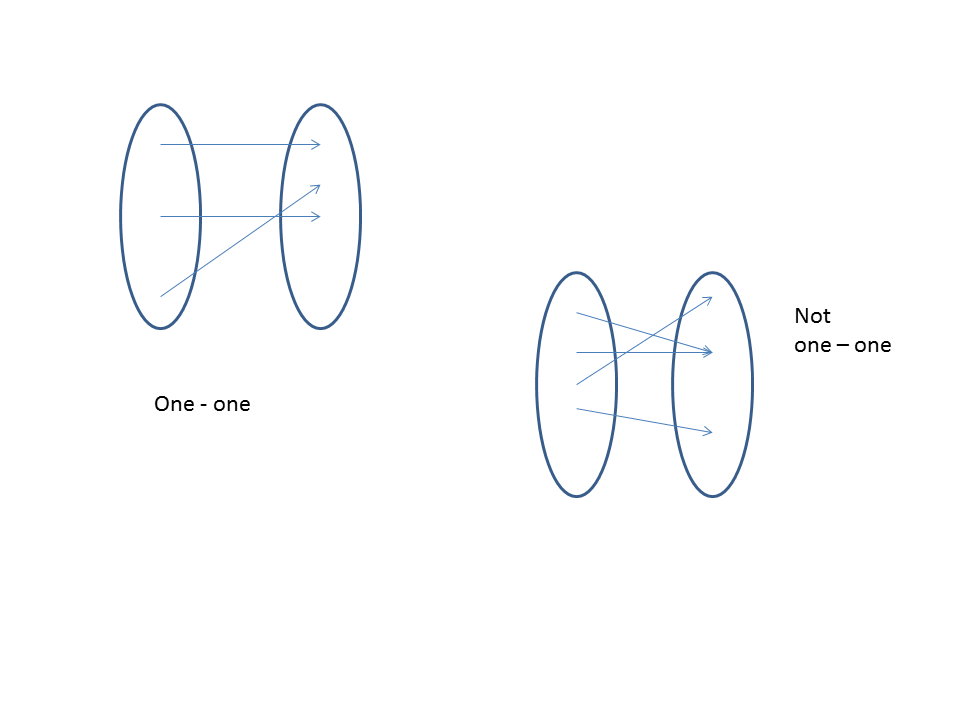
\includegraphics[scale=0.6]{./img/oneone.png}

Example

Is the function $f(x) = x^2$ one-one when the domain and co-domain are the set of real numbers?

Not one-one. For example $f(1) =  f(-1)$, but obviously 1 is not equal to -1.

Is the same function one-one when the domain and co-domain are the set of natural numbers?

Now the function is one-one because 

\begin{align*}
x^2 = y^2 \\
& \implies x^2 - y^2 = 0 \\
& \implies (x - y) (x + y) = 0\\
& \implies x = y \text{ or }  x = -y
\end{align*}

But both $x$ and $y$ are natural numbers and therefore are positive so it must be the case that $x = y$. Therefore the function is one to one.

\section*{Onto}
A function is said to be onto if the entire co-domain is `covered'. More formally, $f:X \rightarrow Y$ will be onto if for every $y \in Y$, there is some $x \in X$ such that $f(x) = y$. 

From an arrow-diagram perspective it just means that there is some arrow incident on every single point in the co-domain.

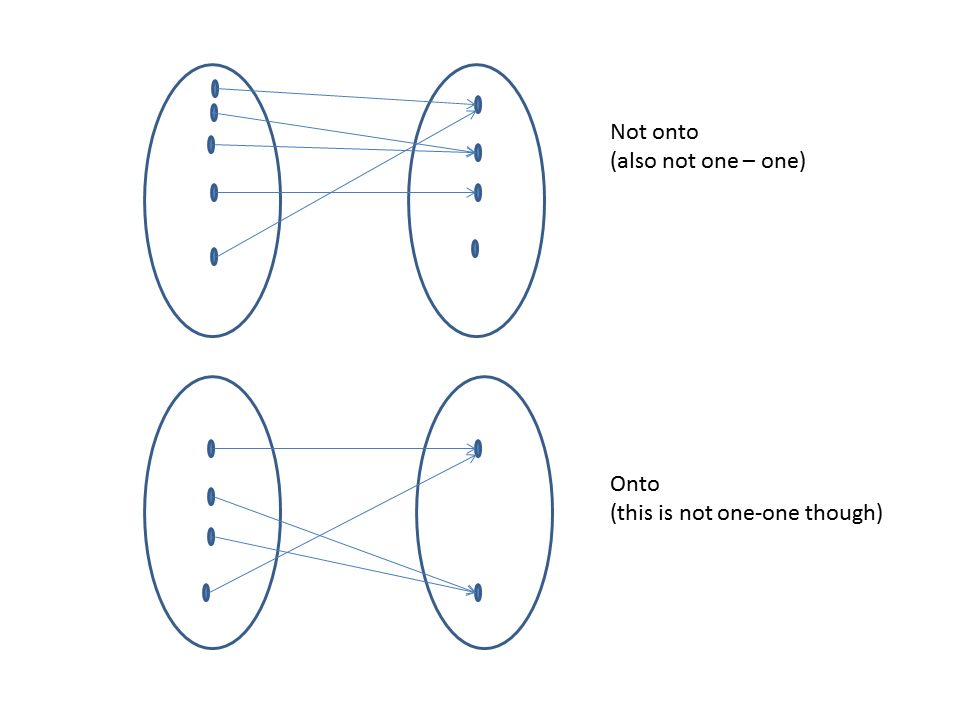
\includegraphics[scale=0.7]{./img/Onto.png}

\vspace{0.5in}

For instance, the function $f: \mathbb{Z} \rightarrow \mathbb{Z} \text{ defined as } f(x) = x^2$ is not onto.
Why?

Is there any integer whose square is equal to 2? 


\section*{Bijection}

A function that is both one to one and onto. 

Examples- 

Let $F = \{`Arvind', `Nitay', `Olivia'\}$ and 

Let $L = \{`Bhusnurmath', `Caspi', `Sun'\}$.

Every first name can be mapped to a unique last name. Also there is no last name that nothing is mapped to.

\medskip

If $f: X \rightarrow Y$ is a bijection from $X$ to $Y$, what can you say about $|X|$ and $|Y|$.

$|X| = |Y|$.


Do not worry about a rigorous proof of that statement yet. Just understand it intuitively as follows. 


Bijection means both onto and one-one. As a consequence of being onto, every element of $Y$ has some arrow incident on it. This immediately means $|X| \ge |Y|$ ($f$ is a function so two arrows cannot come out of the same point in $X$).

As a consequence of being one-one, every element of $X$ has to shoot an arrow to a different element of $Y$. That immediately means $|Y| \ge |X|$. 

Put everything together and you get $|X| = |Y|$.

\section*{Application of bijections}

If you have a bijection between 2 sets you can use elements of one set to exactly represent the other.

If you have seen binary numbers, you know that every positive integer can be expressed in binary, which can basically be considered as a string of 0s and 1s. 

Encoding and decoding are also examples of bijections. You can think of an encoding as the application of a function to the message in order to produce a message that is hard to decipher. Given a secret message, you would want your decoding to be unique otherwise the ambiguity would be annoying.


\end{document}



